\documentclass[]{article}
\usepackage{lmodern}
\usepackage{amssymb,amsmath}
\usepackage{ifxetex,ifluatex}
\usepackage{fixltx2e} % provides \textsubscript
\ifnum 0\ifxetex 1\fi\ifluatex 1\fi=0 % if pdftex
  \usepackage[T1]{fontenc}
  \usepackage[utf8]{inputenc}
\else % if luatex or xelatex
  \ifxetex
    \usepackage{mathspec}
  \else
    \usepackage{fontspec}
  \fi
  \defaultfontfeatures{Ligatures=TeX,Scale=MatchLowercase}
\fi
% use upquote if available, for straight quotes in verbatim environments
\IfFileExists{upquote.sty}{\usepackage{upquote}}{}
% use microtype if available
\IfFileExists{microtype.sty}{%
\usepackage{microtype}
\UseMicrotypeSet[protrusion]{basicmath} % disable protrusion for tt fonts
}{}
\usepackage[margin=1in]{geometry}
\usepackage{hyperref}
\hypersetup{unicode=true,
            pdftitle={Floodrisk and race in Washington},
            pdfauthor={Ailene Ettinger, ailene.ettinger@tnc.org},
            pdfborder={0 0 0},
            breaklinks=true}
\urlstyle{same}  % don't use monospace font for urls
\usepackage{graphicx}
% grffile has become a legacy package: https://ctan.org/pkg/grffile
\IfFileExists{grffile.sty}{%
\usepackage{grffile}
}{}
\makeatletter
\def\maxwidth{\ifdim\Gin@nat@width>\linewidth\linewidth\else\Gin@nat@width\fi}
\def\maxheight{\ifdim\Gin@nat@height>\textheight\textheight\else\Gin@nat@height\fi}
\makeatother
% Scale images if necessary, so that they will not overflow the page
% margins by default, and it is still possible to overwrite the defaults
% using explicit options in \includegraphics[width, height, ...]{}
\setkeys{Gin}{width=\maxwidth,height=\maxheight,keepaspectratio}
\IfFileExists{parskip.sty}{%
\usepackage{parskip}
}{% else
\setlength{\parindent}{0pt}
\setlength{\parskip}{6pt plus 2pt minus 1pt}
}
\setlength{\emergencystretch}{3em}  % prevent overfull lines
\providecommand{\tightlist}{%
  \setlength{\itemsep}{0pt}\setlength{\parskip}{0pt}}
\setcounter{secnumdepth}{0}
% Redefines (sub)paragraphs to behave more like sections
\ifx\paragraph\undefined\else
\let\oldparagraph\paragraph
\renewcommand{\paragraph}[1]{\oldparagraph{#1}\mbox{}}
\fi
\ifx\subparagraph\undefined\else
\let\oldsubparagraph\subparagraph
\renewcommand{\subparagraph}[1]{\oldsubparagraph{#1}\mbox{}}
\fi

%%% Use protect on footnotes to avoid problems with footnotes in titles
\let\rmarkdownfootnote\footnote%
\def\footnote{\protect\rmarkdownfootnote}

%%% Change title format to be more compact
\usepackage{titling}

% Create subtitle command for use in maketitle
\providecommand{\subtitle}[1]{
  \posttitle{
    \begin{center}\large#1\end{center}
    }
}

\setlength{\droptitle}{-2em}

  \title{Floodrisk and race in Washington}
    \pretitle{\vspace{\droptitle}\centering\huge}
  \posttitle{\par}
    \author{Ailene Ettinger,
\href{mailto:ailene.ettinger@tnc.org}{\nolinkurl{ailene.ettinger@tnc.org}}}
    \preauthor{\centering\large\emph}
  \postauthor{\par}
      \predate{\centering\large\emph}
  \postdate{\par}
    \date{2/3/2020}


\begin{document}
\maketitle

\hypertarget{question}{%
\subsection{Question}\label{question}}

Are there racial inequities in floodrisk in Washington state?

\hypertarget{approach}{%
\subsection{Approach}\label{approach}}

Mathis has pulled together an enormous amount of work pulling together
floodrisk and census data to get parcel-level race probabilites for the
entire state of Washington (summarized in the README/technical
document). He has already made a great story board, and figures as well.

I am helping with the statistical models and moving the writing along.

\hypertarget{statistical-models}{%
\subsection{Statistical models}\label{statistical-models}}

Data are grouped into nested levels of blocks, block groups, tracts,
counties, and states. Socioeceonomic level exist only at the tract
level. We have race (probability) at the parcel level.

We fit a multinomial mixed model with the following variables:
-Response: Race (parcel level), multinomial distribution -Predictor:
Flood Status, at the block level -Random effect: county

We fit a multinomial logit model, in which we assume that the log-odds
of each response (proportion of people in each race category) follows a
linear model:
\[\eta_{i,j} = log (\pi_{i,j}/ \pi_{i,J}) = \alpha_{county[i]} + \beta_{flood}  x_{i} + \epsilon_{i}\]\\
\[
\epsilon \sim N(0,\sigma^2_y)
\] \[
\alpha_{county[i]} \sim N(\mu_{\alpha},\sigma^2_{\alpha})
\] where \(\eta\) is race in parcel \emph{i}, \(\alpha_{county[i]}\) is
the county-specific intercept for race \emph{j}, and \emph{x} is flooded
status (0,1) of parcel \emph{i}.

We implement the model in Stan via the brms package.

I'm not sure which model structures we ideally want:

\begin{enumerate}
\def\labelenumi{\arabic{enumi})}
\tightlist
\item
  Random intercept (as shown in the equation, allowing for mean
  differences in floodrisk by county, but assuming the effect of
  floodrisk to be consistent across counties) brms: mod \textless- brm
  (race \textasciitilde{} floodrisk + (1\textbar county), data=wadat,
  family=``multninomial'', prior=c(set\_prior (``normal (0, 1)'')))
\end{enumerate}

or

\begin{enumerate}
\def\labelenumi{\arabic{enumi})}
\setcounter{enumi}{1}
\tightlist
\item
  Random slopes and intercepts (allowing for mean differences in
  floodrisk by county and allowing the effect of floodrisk on race to
  vary across counties). brms: mod \textless- brm (race
  \textasciitilde{} floodrisk + (floodrisk\textbar county), data=wadat,
  family=multinomial(), prior=c(set\_prior (``normal (0, 1)''))) \#\#
  Progress I fit a single level version of the model to a single county
  and for 5 counties. The multi-level version is currently running on
  the 5-county subset. It takes forever currently so I need to get it to
  run more efficiently before fitting to the full dataset (structure of
  the random effects, adding priors) to help it run more efficiently.
\end{enumerate}

The single level model fits well

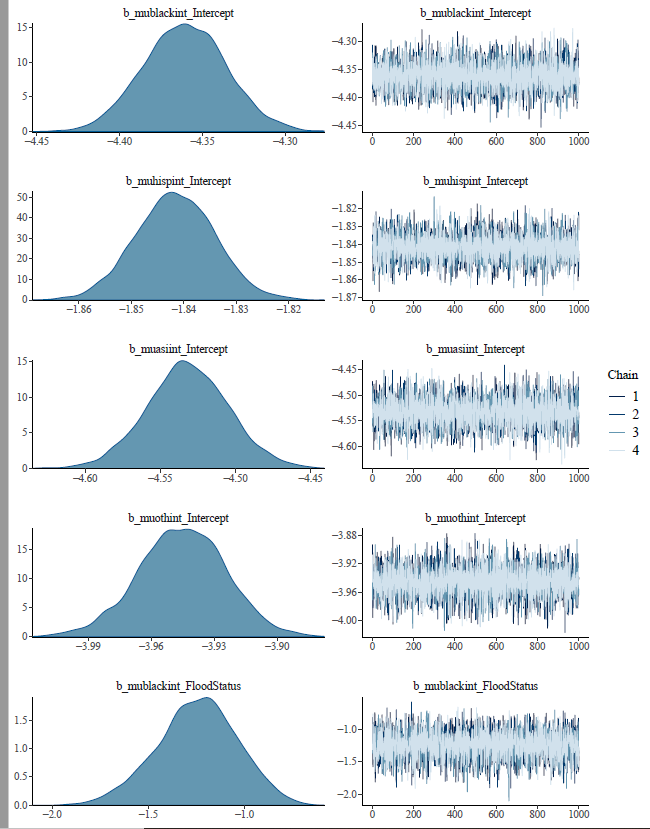
\includegraphics{figures/5counties_modplot.PNG}

It suggests that as floodrisk increases, the probability of whites
inhabiting a parcel increases and the probability of hispanics
increases.

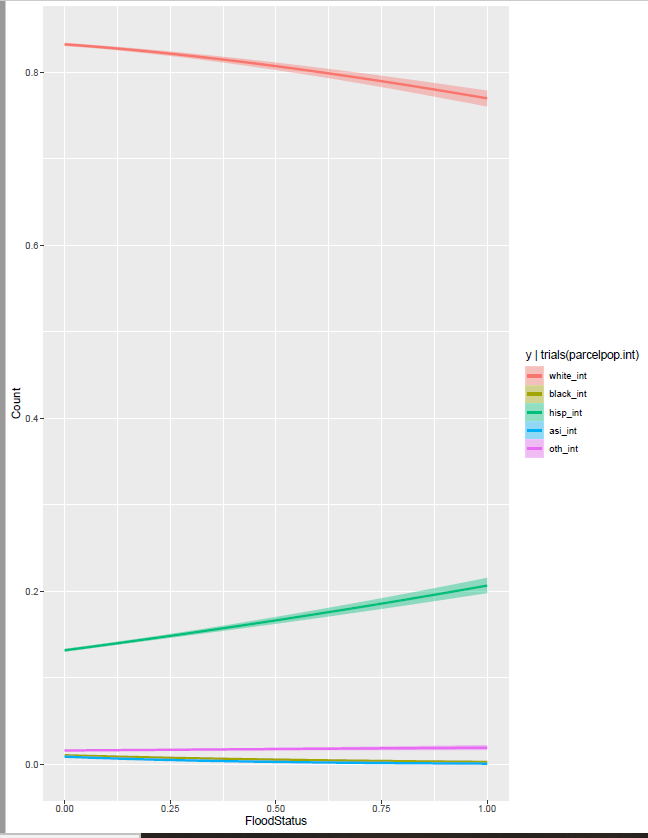
\includegraphics{figures/5counties_condeff_noprior.png}

\hypertarget{next-steps}{%
\subsection{Next Steps}\label{next-steps}}

\begin{enumerate}
\def\labelenumi{\arabic{enumi})}
\tightlist
\item
  Fit multi-level model with county (using reduced dataset)
\item
  Fit multi-level model with county (using full dataset)
\item
  Outline/writing
\end{enumerate}

\hypertarget{notes-and-resources}{%
\subsection{Notes and Resources}\label{notes-and-resources}}

Helpful links and code:

\url{https://cran.r-project.org/web/packages/brms/vignettes/brms_multivariate.html}

\url{https://stackoverflow.com/questions/21082396/multinomial-logistic-multilevel-models-in-r}

\url{https://data.princeton.edu/wws509/notes/c6s2}


\end{document}
